\documentclass[fonset = fandol]{ctexart}
\usepackage{graphicx}
\usepackage[showframe]{geometry}
\usepackage{subfig}
% 关于子图的交叉引用,参考 https://tex.stackexchange.com/questions/75014/is-it-possible-to-make-a-reference-to-a-subfigure-to-appear-figure-2a-with-cle
%\captionsetup[subfigure]{subrefformat=simple,labelformat=simple,listofformat=subsimple}
%\renewcommand\thesubfigure{(\alph{subfigure})}

\begin{document}
\begin{figure}
	\centering
	\subfloat[示例图片1]{\label{fig1}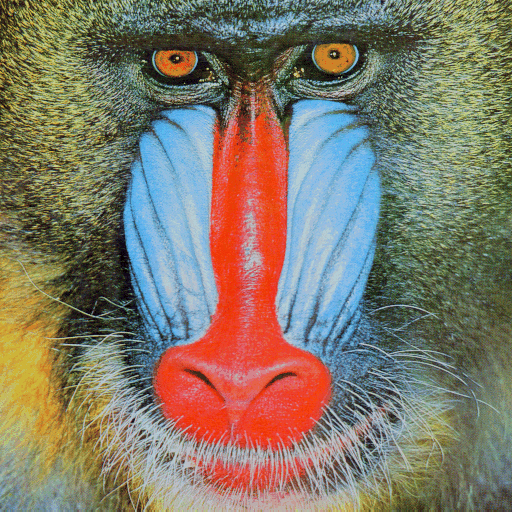
\includegraphics[width=0.48\linewidth]{image1}}
	\hfill
	\subfloat[示例图片2]{\label{fig2}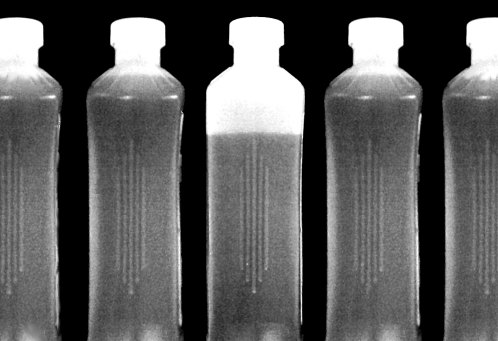
\includegraphics[width=0.48\linewidth]{image2}}
	\caption{两个图片并排,使用子题注} \label{fig3}
\end{figure}
图 \ref{fig1} 和 \ref{fig2} 是图 \ref{fig3} 的子图.
\end{document}